% See: https://latexdraw.com/draw-flowcharts-latex-tutorial/
% See: https://tex.stackexchange.com/questions/51757/how-can-i-use-tikz-to-make-standalone-svg-graphics
\documentclass[crop,tikz,convert={outext=.svg,command=\unexpanded{pdf2svg \infile\space../assets/\outfile}},multi=false]{standalone}

% Required packages
\usepackage{tikz}
\usetikzlibrary{shapes, arrows, calc, positioning}

\begin{document}

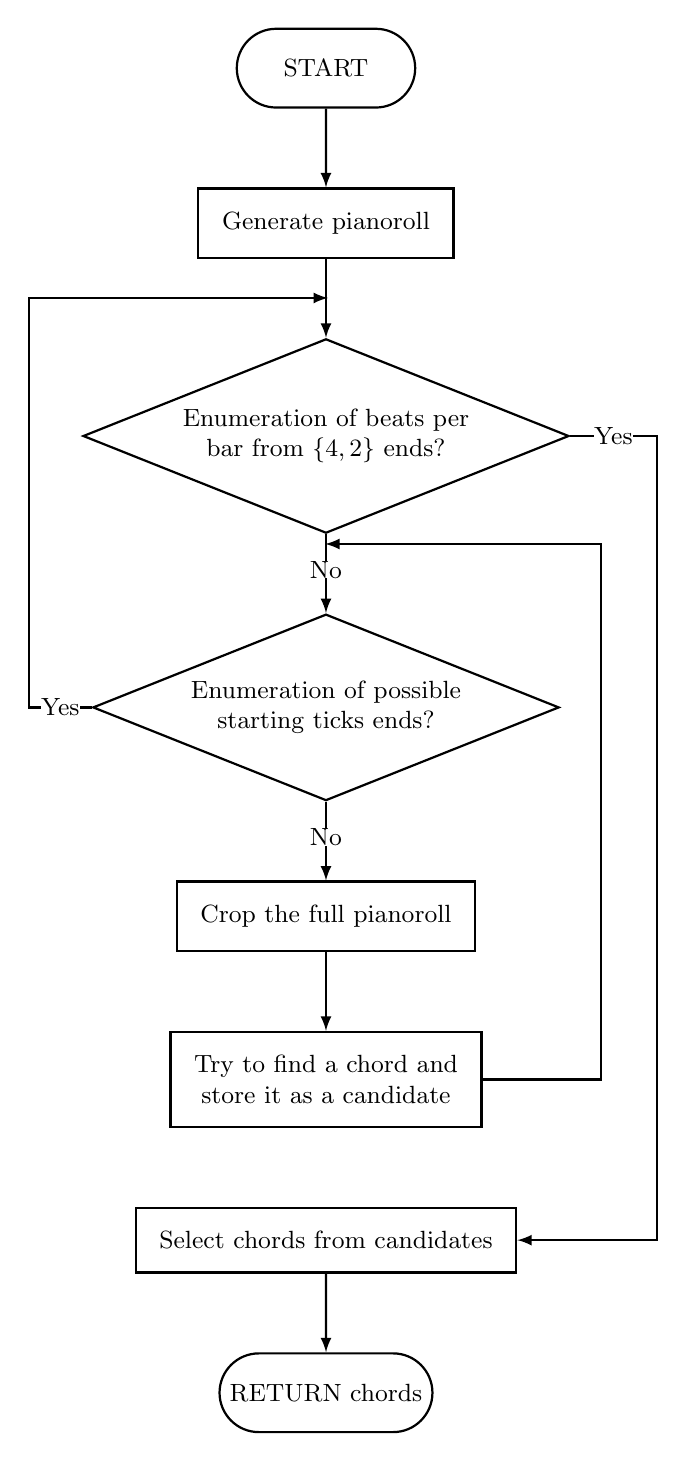
\begin{tikzpicture}[font=\small,thick]

\node[draw,
    rounded rectangle,
    minimum width=2.5cm,
    minimum height=1cm] (block1) {START};

\node[draw,
    align=center,
    below=of block1,
    inner sep=0.3cm] (block2) {Generate pianoroll};

\node[draw,
    diamond,
    below=of block2,
    aspect=2.5,
    align=center,
    minimum width=1cm,
    minimum height=1cm] (block3) {Enumeration of beats per \\ bar from $\{4,2\}$ ends?};

\node[draw,
    diamond,
    below=of block3,
    aspect=2.5,
    align=center,
    minimum height=1cm] (block4) {Enumeration of possible \\ starting ticks ends?};

\node[draw,
    align=center,
    below=of block4,
    inner sep=0.3cm] (block5) {Crop the full pianoroll};

\node[draw,
    align=center,
    below=of block5,
    minimum width=2.5cm,
    inner sep=0.3cm] (block6) {Try to find a chord and \\ store it as a candidate};

\node[draw,
    align=center,
    below=of block6,
    inner sep=0.3cm] (block7) {Select chords from candidates};

\node[draw,
    rounded rectangle,
    below=of block7,
    minimum width=2.5cm,
    minimum height=1cm] (block8) {RETURN chords};

\draw[-latex] (block1) -- (block2);
\draw[-latex] (block2) -- (block3);
\draw[-latex] (block5) -- (block6);
\draw[-latex] (block7) -- (block8);

\draw[-latex] (block3) -- (block4)
    node (no1) [pos=0.45,fill=white,inner sep=0]{No};
\draw[-latex] (block4) -- (block5)
    node (no2) [pos=0.45,fill=white,inner sep=0]{No};

\draw[-latex] (block6.east) -- +(1.5cm,0) |- +(-2cm,6.8cm);
\draw[-latex] (block4.west) -- +(-0.8cm,0)
    node[pos=0.5,fill=white,inner sep=0]{Yes} |- +(3cm,5.2cm);
\draw[-latex] (block3.east) -- +(1.1cm,0)
    node[pos=0.5,fill=white,inner sep=0]{Yes} |- (block7.east);

\end{tikzpicture}

\end{document}
